\documentclass[a4,11pt]{article}
\topmargin = 2pt
\textwidth = 450pt
\textheight = 640pt
\marginparwidth = 90pt
\evensidemargin = 54pt

\usepackage[usenames,dvipsnames]{xcolor}
\usepackage{enumerate}
\usepackage{multicol}
\usepackage[showframe=false, margin=0.5in]{geometry}
\usepackage{changepage}

\usepackage{lipsum}   % for filler text
\usepackage{afterpage}
\usepackage{graphicx}
\usepackage{version}
\usepackage{enumitem}
\usepackage{listings}
\lstdefinestyle{Bash}
{language=bash,
keywordstyle=\color{blue},
basicstyle=\ttfamily,
morekeywords={peter@kbpet},
alsoletter={:~\$},
morekeywords=[2]{ak2@ak2-XPS-L501X:},
keywordstyle=[2]{\color{red}},
literate={\$}{{\textcolor{red}{\$}}}1 
         {:}{{\textcolor{red}{:}}}1
         {~}{{\textcolor{red}{\textasciitilde}}}1,
}

\includeversion{question}\includeversion{solution}
\setlist[description]{style=nextline}

\newenvironment{que}
{ \color{YellowGreen}
  \begin{question}
}
{ \end{question} }

\newenvironment{sol}
{ \color{Black}
  \begin{solution}
}
{ \end{solution} }


\begin{document}

\title{CS349 : Networks Lab \\
	Report\\
	Assignment 3: Wireshark}
\author{Anil Kag\\
	   10010111\\
	   a.kag@iitg.ernet.in}
\date{March 20, 2013}
\maketitle


\section{Basics}
	  
\begin{enumerate}
 %prb 1%
 \item
  \begin{que}
    List up to 10 different protocols that appear in the protocol column in the unfiltered packet-listing window in step 7 above. 
  \end{que}
   
  \begin{sol}
   \textbf{Ans:} Protocols which appear in the protocol column in the unfiltered packet-listing
      \begin{multicols}{3}
	\begin{enumerate}
	\item ARP  	\item DHCiPv6
	\item DNS 	\item Ethernet 
	\item ICMP      	\item HTTP
	\item LLC        \item LLMNR
	\item SSDP       \item STP 
	\item TCP       	\item UDP
	\end{enumerate}
      \end{multicols}
    \end{sol}
    
    
    %prb 2%
    \item
    \begin{que} 
      How long did it take from when the HTTP GET message was sent until the HTTP OK reply was received? 
    \end{que}

    \begin{sol}
      \textbf{Ans:} Packet details are as follows \\
      \begin{tabular}{|r|l|l|l|l|l| p{10cm} |}
       \hline
       no&	time&			source&			destination&		proto&	len&	info \\
       \hline
       310& 	17:00:18.753711& 	172.16.27.59& 		202.141.80.22& 		HTTP& 	867& 	GET http://www.google.co.in/ HTTP/1.1 \\
       391& 	17:00:18.903545&	202.141.80.22&		172.16.27.59&		HTTP&	66&	HTTP/1.0 200 OK  (text/html)\\
       \hline
      \end{tabular}

      Time taken = $0.903545sec-0.753711 sec = 0.149834 sec$
    \end{sol}
 
      %prb 3%
      \item
      \begin{que}
	What is the Internet address of the www.google.com? What is the Internet address of your computer? 
      \end{que}
      
      \begin{sol}
	\textbf{Ans:} IP of google cannot be determined by looking at the above two packets because the proxy server(202.141.80.22) handles
	the connection part between my host \& google.com. Firstly my machine tries to resolve the domain name ``www.google.com''
	but the dns server fails in resolving the address \& hence the packet is sent to the proxy server which then handles 
	the connection for interacting with public addresses.\\
	My host ip $\Rightarrow$ 172.16.27.59 (can be seen in the src field in IP header in http get request)
      \end{sol}
\end{enumerate}
\pagebreak 


\section{Ethernet}
	 
    \textit{Reference packets used for solving this part}\\
      \begin{tabular}{|r|l|l|l|l|l| p{6cm} |}
       \hline
       no&	time&			source&			destination&		proto&	len&	info \\
       \hline
       113& 	17:47:02.684944& 	172.16.27.59& 		202.141.80.22& 		HTTP& 	668& 	GET http://www.faqs.org/rfcs/rfc826.html HTTP/1.1 \\
       391& 	17:47:03.771542&	202.141.80.22&		172.16.27.59&		HTTP&	3935&	HTTP/1.0 200 OK  (text/html)\\
       \hline
      \end{tabular}
	  
\begin{enumerate}
  %prb 1%
  \item 
  \begin{que}
   What is the 48-bit Ethernet address of your computer?
  \end{que}

  \begin{sol}
    \textbf{Ans:} HTTP GET message's ethernet header \\
      Ethernet II, Src: Pegatron\_b3:05:c4 (38:60:77:b3:05:c4), Dst: Cisco\_9d:70:00 (00:24:f9:9d:70:00) \\
      Ethernet address of my computer	 Pegatron\_b3:05:c4 ( 38:60:77:b3:05:c4) given by src field
  \end{sol}

  
   %prb 2%
   \item
   \begin{que}
    What is the 48-bit destination address in the Ethernet frame? 
    Is this the Ethernet address of the website with the RFC?  What device has this as its Ethernet address?
   \end{que}

   \begin{sol}
      \textbf{Ans:} Destination Ethernet address 		00:24:f9:9d:70:00	\\

      It's not the ethernet address of the RFC website. \\
      It's actually the ethernet address of the next hop for reaching the destination in my computer's routing table. \\

      You can actually check the IP for the device having destination ethernet address as this by 
      running 'arp -n' on your linux machine \& check the IP corresponding to this ethernet address on my machine.
    \begin{adjustwidth}{-2cm}{}
      \begin{lstlisting}[style=bash]
      $ arp -n
      Address     	HWtype  HWaddress           Flags Mask   Iface
      172.16.27.68       ether   f0:4d:a2:4f:15:6d   C            eth0
      172.16.24.254      ether   00:24:f9:9d:70:00   C            eth0
      \end{lstlisting}
      \end{adjustwidth}
      
      $\Rightarrow$ it's ethernet address of 172.16.24.254
   \end{sol}

  %prb3%
  \item
  \begin{que}
   Give the hexadecimal value for the two-byte Frame type field. What do the bit(s) whose value is 1 mean within the flag field?
  \end{que}
  
  \begin{sol}
   \textbf{Ans:} Type field value = 0x0800 $\Rightarrow$ IP packet \\
	    There are no flags in the Ethernet II header.
  \end{sol}
  
  % prb 4 %
  \item 
  \begin{que}
   How many bytes from the very start of the Ethernet frame does the ASCII “G” in “GET” appear in the Ethernet frame?
  \end{que}

  \begin{sol}
   \textbf{Ans:} Ethernet Header Contents
   \begin{adjustwidth}{-2cm}{}
    \begin{lstlisting}[style=bash]
      0000  00 24 f9 9d 70 00 38 60  77 b3 05 c4 08 00 45 00   .$..p.8` w.....E.
      0010  02 8e 56 bd 40 00 40 06  ff bd ac 10 1b 3b ca 8d   ..V.@.@. .....;..
      0020  50 16 c9 6a 0c 38 94 40  d2 f1 66 42 57 69 80 18   P..j.8.@ ..fBWi..
      0030  00 e5 28 7f 00 00 01 01  08 0a 00 9e 84 4b 15 b1   ..(..... .....K..
      0040  50 ee 47 45 54 20 68 74  74 70 3a 2f 2f 77 77 77   P.GET ht tp://www
    \end{lstlisting}
    \end{adjustwidth}
    
    ASCII letter 'G' starts on line 5 with base $0x0040$ \& offset $0x0003$ \\
    Ethernet Header size = 14bytes \& IP Header size = 20bytes \& TCP Header Size = 32bytes (in my case 12bytes extra is covered by options field) \\
    $\Rightarrow$ position (in bytes) from the start of Ethernet Frame $= 4*16+3 = 67$ ($0x0010 = 16$ in decimal) \\
    i.e. G comes after $14+20+32 = 66$ bytes in the packet   
  \end{sol}

  %prb 5%
  \item 
  \begin{que}
   What is the value of the Ethernet source address? 
   Is this the address of your computer, or of the destination website?  What device has this as its Ethernet address?
  \end{que}

  \begin{sol}
   \textbf{Ans:} HTTP Response \\
    Ethernet II, Src: Cisco\_9d:70:00 (00:24:f9:9d:70:00), Dst: Pegatron\_b3:05:c4 (38:60:77:b3:05:c4) \\
    src = 00:24:f9:9d:70:00 $\Rightarrow$ hop just before my computer in the path from website to my computer  
  \end{sol}
  
  %prb 6%
  \item 
  \begin{que}
   What is the destination address in the Ethernet frame? Is this the Ethernet address of your computer?
  \end{que}

  \begin{sol}
 \textbf{Ans:}   dst = 38:60:77:b3:05:c4 $\Rightarrow$ my computer (you can verify via ifconfig \& look at the hwaddress for the eth0 interface)
    \begin{adjustwidth}{-2cm}{}
    \begin{lstlisting}[style=bash]
      $ ifconfig
      eth0      Link encap:Ethernet  HWaddr 38:60:77:b3:05:c4  
		inet addr:172.16.27.59  Bcast:172.16.27.255  Mask:255.255.252.0
		inet6 addr: fe80::3a60:77ff:feb3:5c4/64 Scope:Link
		UP BROADCAST RUNNING MULTICAST  MTU:1500  Metric:1
		RX packets:8008125 errors:0 dropped:4342 overruns:0 frame:0
		TX packets:173669 errors:0 dropped:0 overruns:0 carrier:0
		collisions:0 txqueuelen:1000 
		RX bytes:1129843477 (1.1 GB)  TX bytes:20988447 (20.9 MB)
		Interrupt:43 Base address:0xe000 

      lo        Link encap:Local Loopback  
		inet addr:127.0.0.1  Mask:255.0.0.0
		inet6 addr: ::1/128 Scope:Host
		UP LOOPBACK RUNNING  MTU:16436  Metric:1
		RX packets:21789 errors:0 dropped:0 overruns:0 frame:0
		TX packets:21789 errors:0 dropped:0 overruns:0 carrier:0
		collisions:0 txqueuelen:0 
		RX bytes:1986523 (1.9 MB)  TX bytes:1986523 (1.9 MB)
    \end{lstlisting}   
    \end{adjustwidth}
  \end{sol}

  %*** prb 7%
  \item
  \begin{que}
    Give the hexadecimal value for the two-byte Frame type field. What do the bit(s) whose value is 1 mean within the flag field?   
  \end{que}

   \begin{sol}
  \textbf{Ans:}  Type field == 0x0800 $\Rightarrow$ IP \\
    There are no flags in the Ethernet II header.   
   \end{sol}
   
\end{enumerate}
\pagebreak


\section{IP}
 \begin{figure}[h!]
      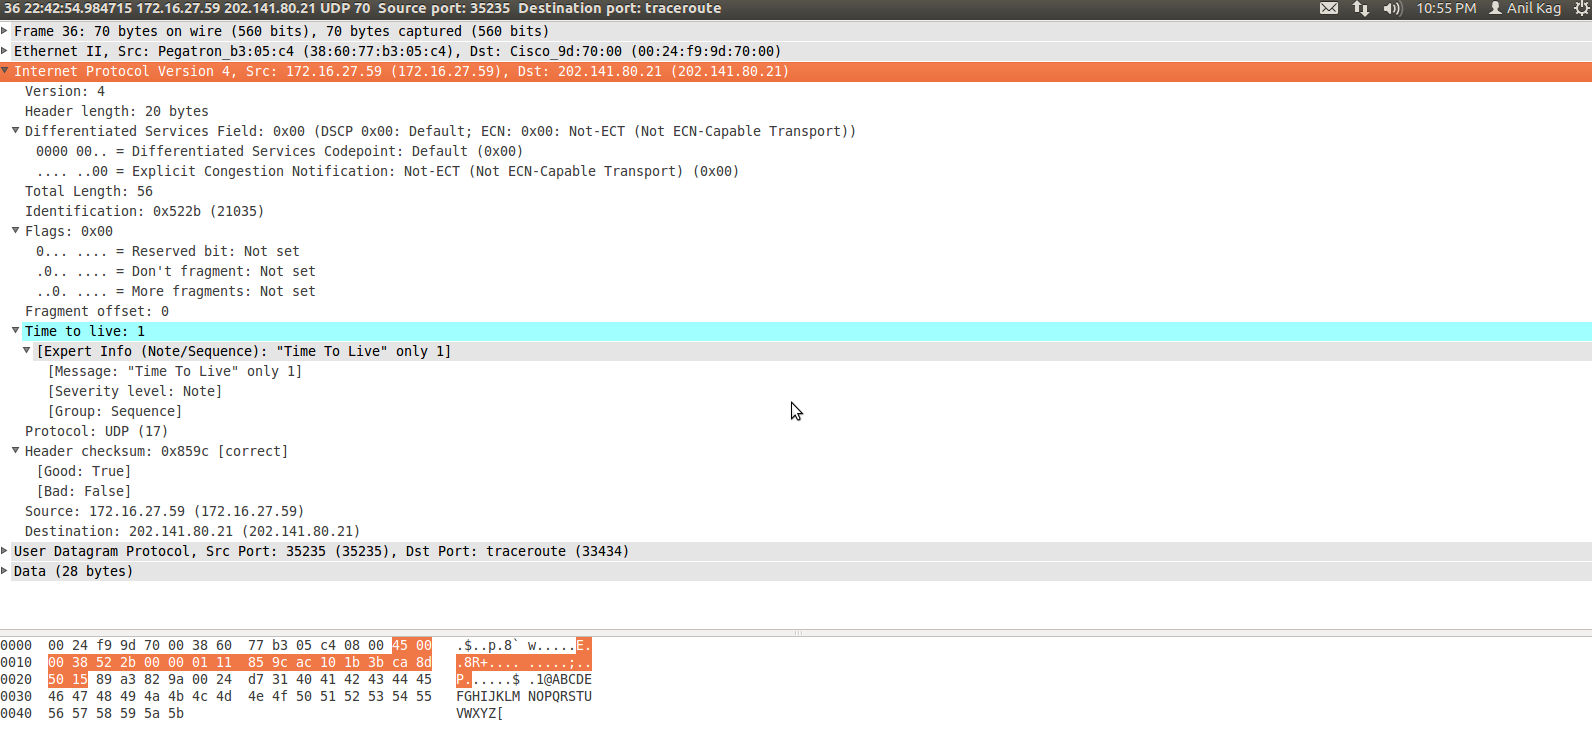
\includegraphics[width=0.9\textwidth]{IP-Header.png}
          \caption{IP Header}
          \label{IP-Header}
  \end{figure}

  \begin{enumerate}
   \item
    \begin{que}
      What is the IP address of your computer?
    \end{que}
    
    \begin{sol}
    \textbf{Ans:}  Internet Protocol Version 4, Src: 172.16.27.59 (172.16.27.59), Dst: 202.141.80.21 (202.141.80.21) \\
	$\Rightarrow$  IP of my computer = 172.16.27.59    
    \end{sol}

   
    \item
      \begin{que}
	Within the IP packet header, what is the value in the upper layer protocol field?
      \end{que}
      
      \begin{sol}
      \textbf{Ans:} 	Protocol: UDP (17)
      \end{sol}

      
    \item
      \begin{que}
	How many bytes are in the IP header? How many bytes are in the payload of the IP datagram? 
	Explain how you determined the number of payload bytes.
      \end{que}
      
      \begin{sol}
	 \textbf{Ans:} Internet Header Length = 20bytes \\
	(if only looking at packet, value given in IHLen is 5 $\Rightarrow 5*32$ bits = $5*4$bytes = 20 bytes) \\
	
	Total Length = 56bytes = Header Length + IP Payload Length \\
	$\Rightarrow$ IP Payload Length = 56bytes - 20bytes = 36bytes \\
	(as Header length = 20bytes)
      \end{sol}

     \item
      \begin{que}
	 Has this IP datagram been fragmented? Explain how you determined whether or not the datagram has been fragmented.
      \end{que}
      
      \begin{sol}
	 \textbf{Ans:}   Flags: 0x00 \\
	  0... .... = Reserved bit:   Not set \\
	  .0.. .... = Don't fragment: Not set \\
	  ..0. .... = More fragments: Not set \\
	  Fragment offset: 0 \\
	  Since fragment offset is 0 \& no more fragments are going to come(more bit not set) \\
	  $\Rightarrow$ no fragmentation
      \end{sol}

  \item 
  \begin{que}
   Which fields in the IP datagram always change from one datagram to the next within this series of ICMP messages sent by your computer?
  \end{que}

  \begin{sol}
    \textbf{Ans:} Identification \& Checksum always change while going from one packet to other \\
  \end{sol}
  
  \item
  \begin{que}
    Which fields stay constant? Which of the fields must stay constant? Which fields must change? Why?
  \end{que}

  \begin{sol}
   \textbf{Ans:} 
	Fields which stay constant are Version, Header Length, Differentiated Services, Protocol, Src \& Dest IP. \\
	The field stated above must remain constant, because, version is 4 due to IPv4 \& hence length also is fixed.
	Also the protocol field =  UDP(17). \\
	Field which must change are identification \& checksum (these two may also change depending on certain conditions). \\
	Identification field uniquely identifies a packet \& hence should be unique except for the case of fragmentation.
  \end{sol}

  
  \item
  \begin{que}
   What is the value in the Identification field and the TTL field? 
   Do these values remain unchanged for all of the ICMP TTL-exceeded replies sent to your computer by the nearest (first hop) router? Why?
  \end{que}

  \begin{sol}
  \textbf{Ans:}  
  
   \begin{figure}[h!]
      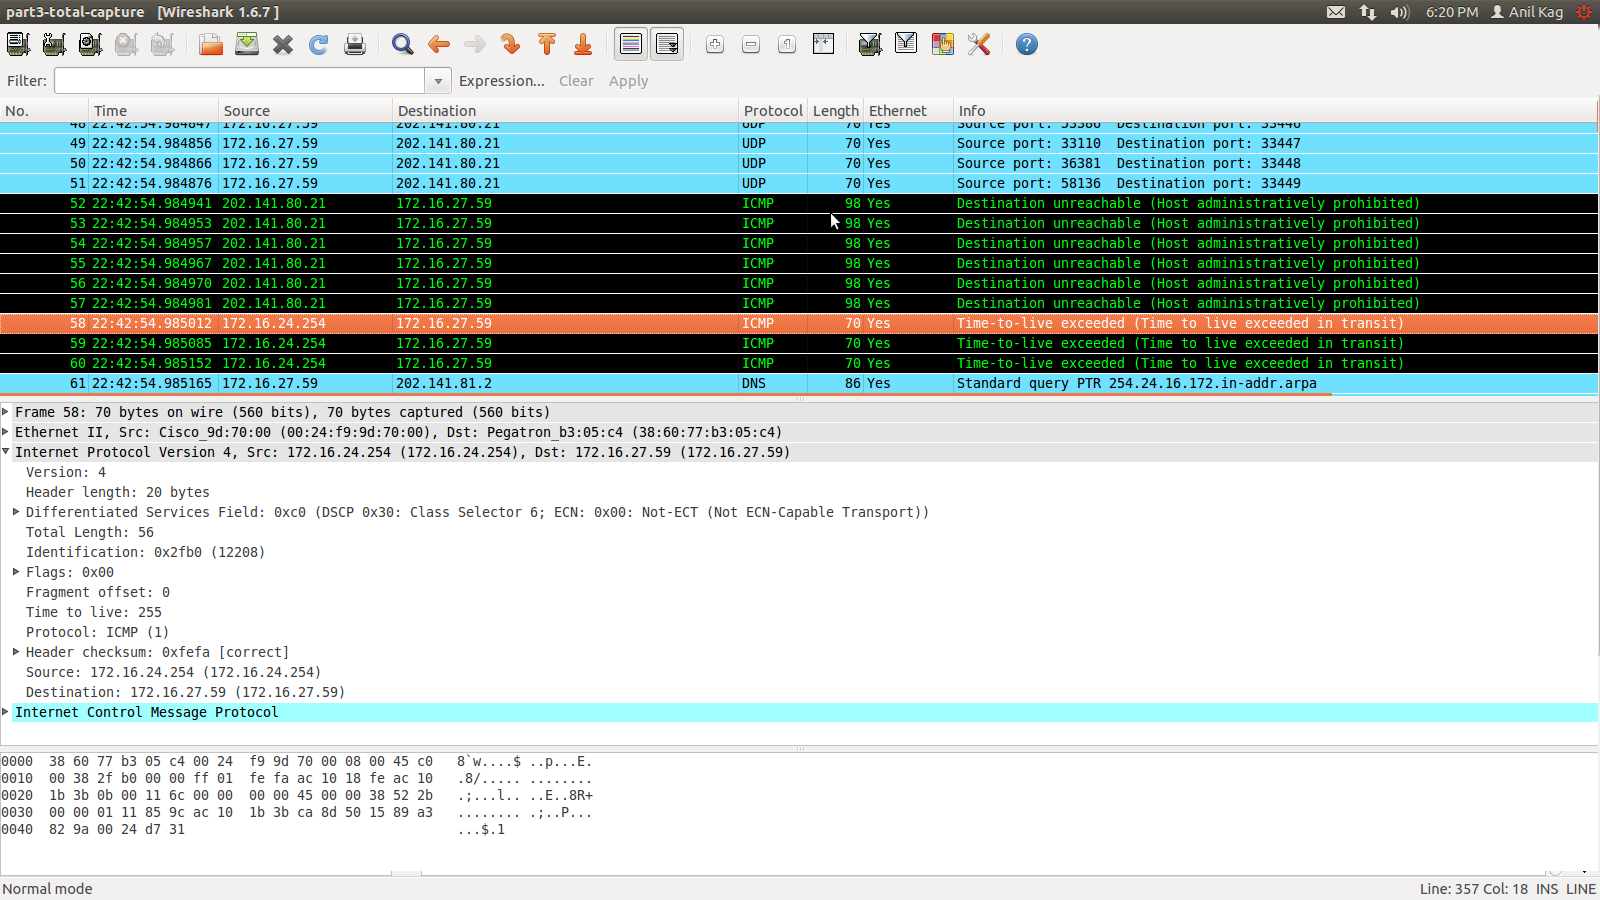
\includegraphics[width=0.9\textwidth]{ttl-values.png}
          \caption{TTL Value \& Id Field}
          \label{TTL}
  \end{figure}
  
    For the current packet (figure ~\ref{TTL}) \\
    Identification: $0x2fb0 (12208)$ \\
    Time to live: $255$ \\
    
    Yes, the TTL values in all these messages remains the same but the identification value changes.
    Since the TTL-Exceeded replies are sent by the nearest router (first hop), the TTL values will be set to maximum of that field which
    means that it'll be $256$ because the TTL field is 8bits long. No other router exists in between my computer \& first hop router \&
    hence no one can reduce the TTL value.\\
    
  \end{sol}
 \end{enumerate}
\pagebreak

\section{UDP}
  \begin{figure}[h!]
      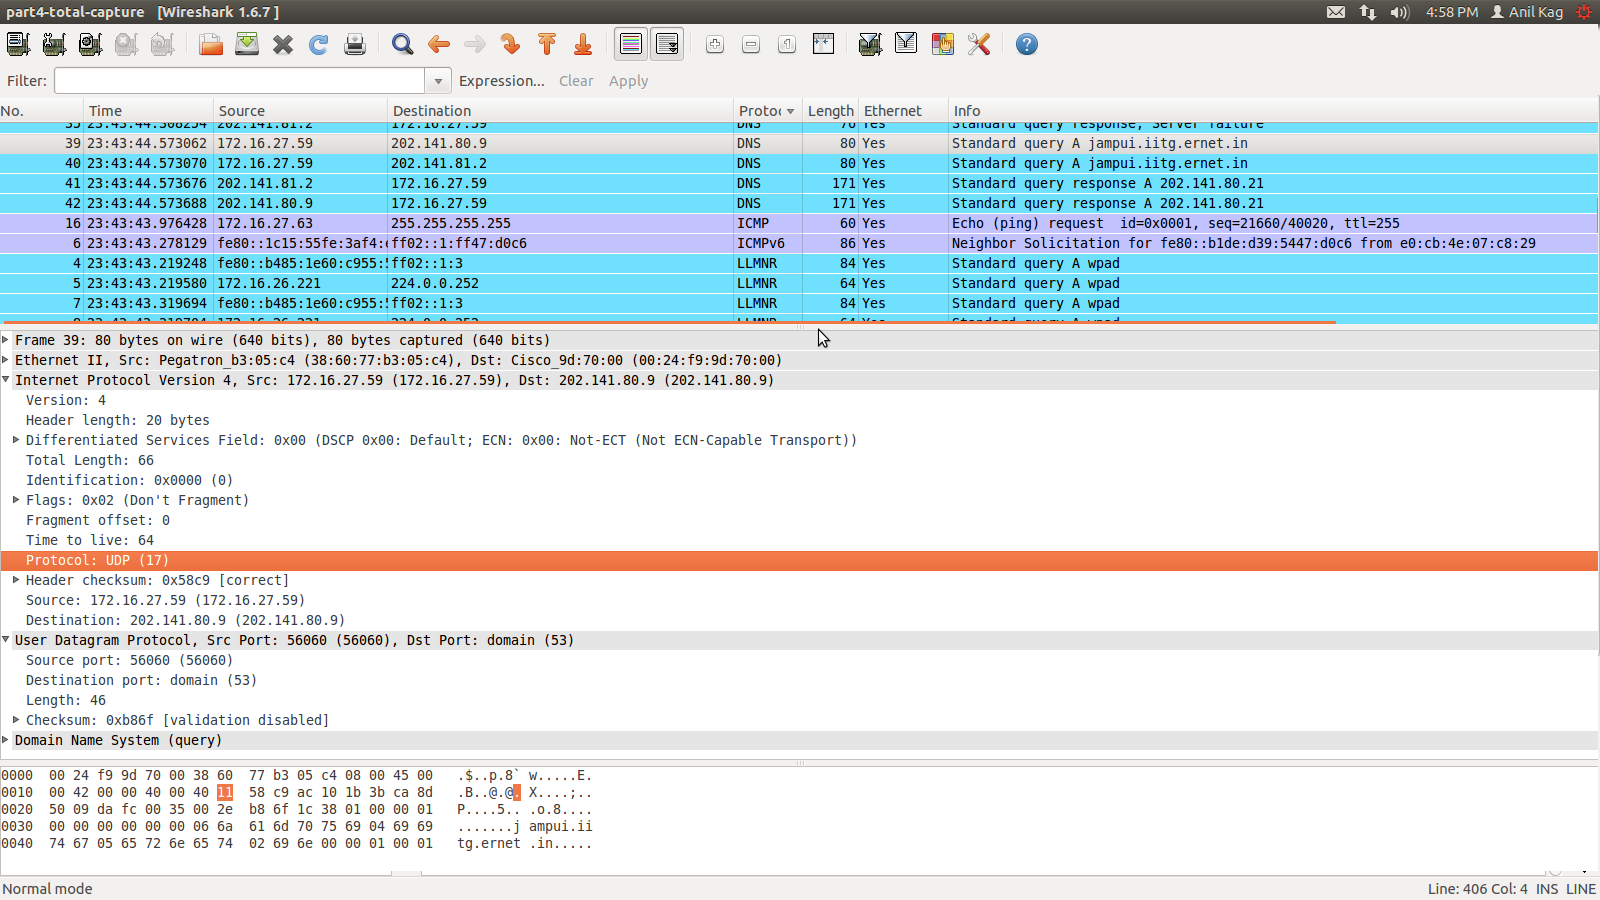
\includegraphics[width=0.9\textwidth]{udp-ip-header.png}
          \caption{UDP Header}
  \end{figure}

       \begin{figure}[h!tb]
      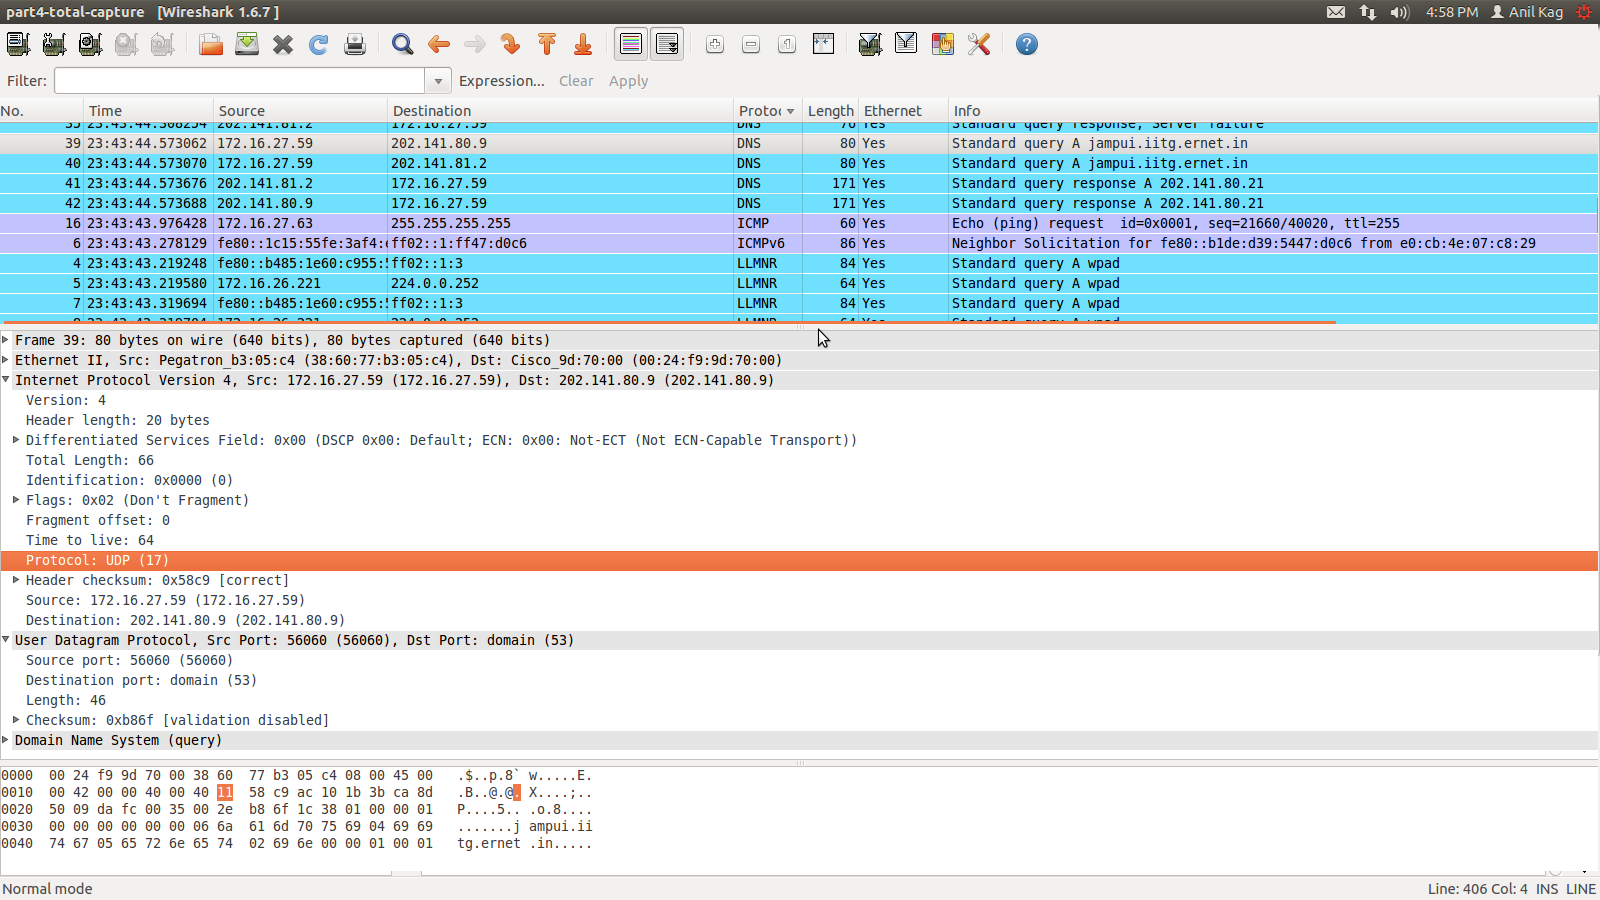
\includegraphics[width=0.9\textwidth]{udp-ip-header.png}
          \caption{UDP+IP Header}
          \label{fig:udp_ip}
  \end{figure}
  
    \begin{figure}[h!tb]
        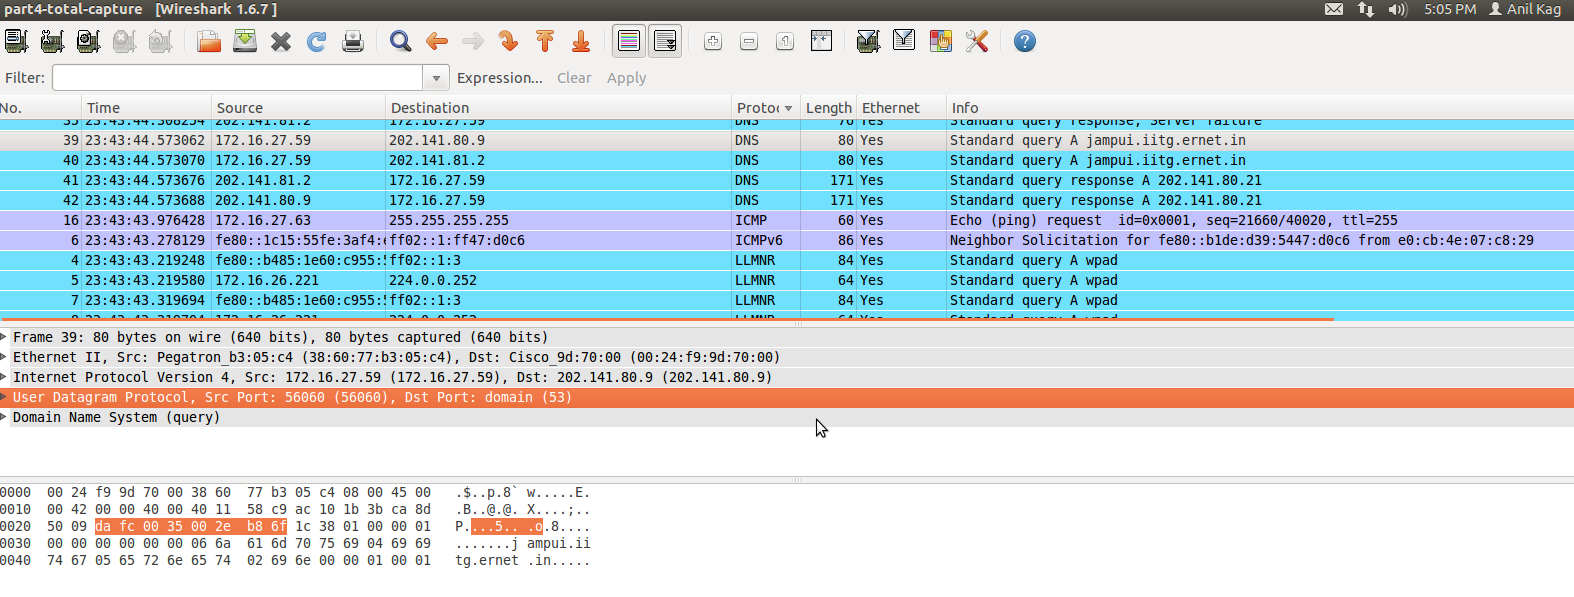
\includegraphics[width=0.9\textwidth]{full-udp-header.png}
          \caption{UDP Header marked} 
          \label{fig:udp_header}
   \end{figure}
   
    \begin{figure}[h!tb]
        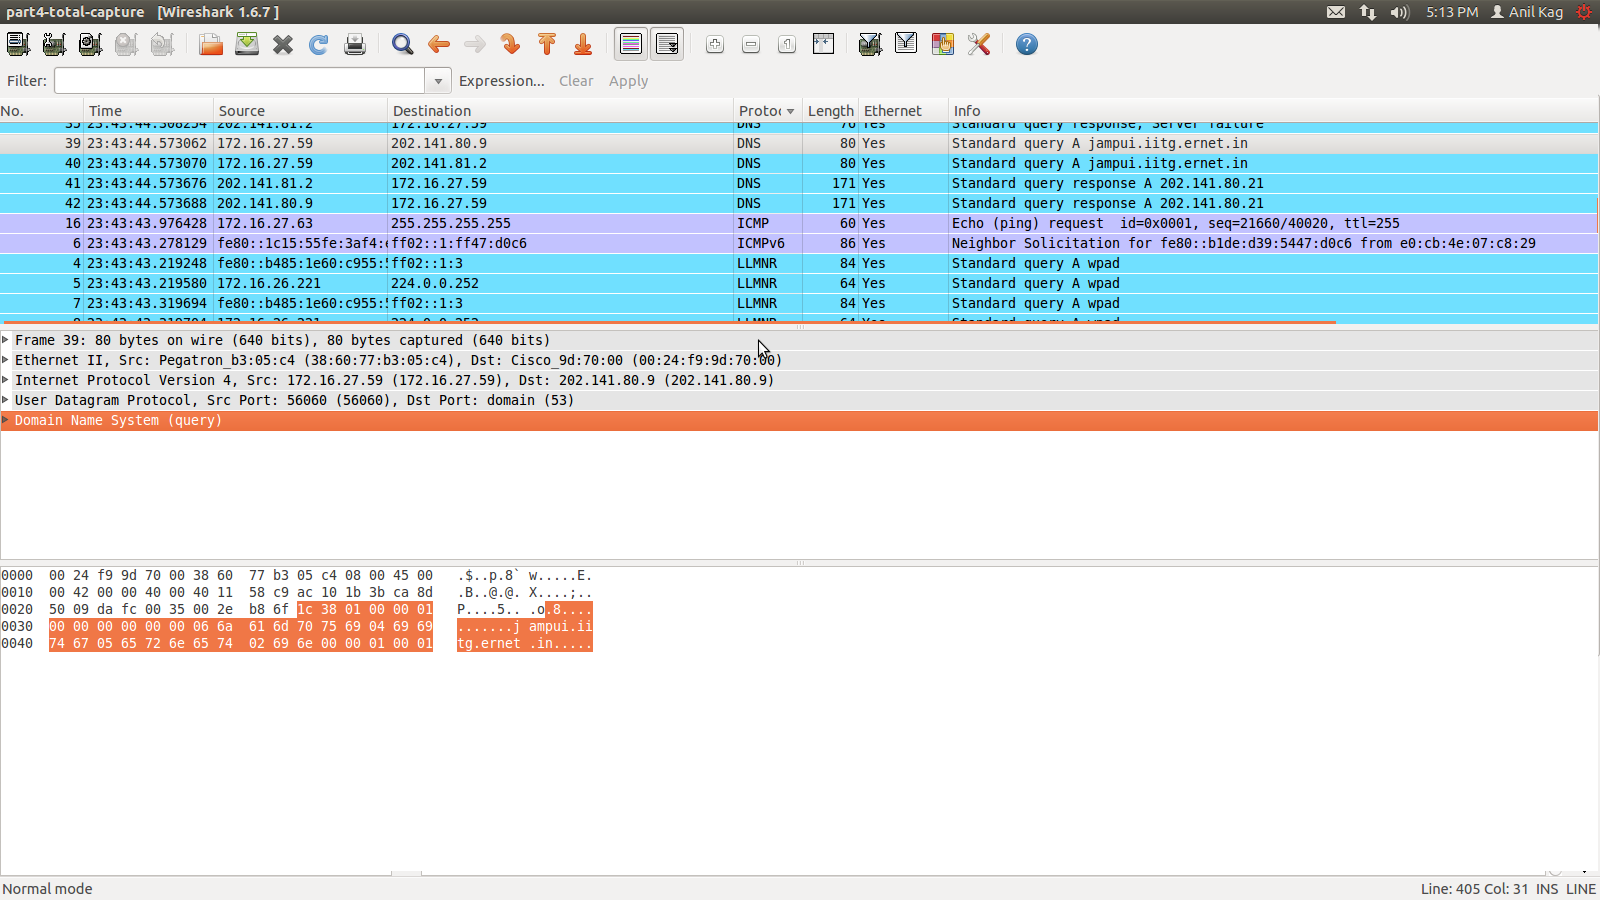
\includegraphics[width=0.9\textwidth]{udp-payload-marked.png}
         \caption{UDP Payload Marked}
         \label{fig:udp_payload}
  \end{figure}
  \pagebreak
  \begin{enumerate}
   \item 
   \begin{que}
    Select one packet. From this packet, determine how many fields there are in the UDPheader. Name these fields.
   \end{que}

   \begin{sol}
   \textbf{Ans:} Fields in the UDP header are as follows (can be seen in the UDP section of the packet): 
   \begin{multicols}{2}
      \begin{enumerate}
	\item source port
	\item destination port
	\item length
	\item checksum
      \end{enumerate}
    \end{multicols} 
   \end{sol}

   
  \item
  \begin{que}
    From the packet content field, determine the length (in bytes) of each of the UDP header fields. 
  \end{que}

  \begin{sol}
   \textbf{Ans:}  Each Field in the UDP Header is 2bytes(16 bits) long $\Rightarrow$ total udp header length = $8bytes$
  \end{sol}
  
  
  \item
  \begin{que}
   The value in the Length field is the length of what? Verify your claim with your captured UDP packet.
  \end{que}

  \begin{sol}
  \textbf{Ans:} Select the DNS query portion \& it expands over 46bytes which is equal to the length given in the UDP packet \\
      $\Rightarrow$ length in UDP packet refers to the payload length along with the UDP header length. \\
         
      UDP Header length $8bytes$. \textit{See figure ~\ref{fig:udp_header} }\\
      Payload length is $2*16 bytes$(in last 2 rows) +$6 bytes$(in 3rd last row)= $38bytes$. \textit{See figure ~\ref{fig:udp_payload}}
   \end{sol} 

   
  \item
  \begin{que}
   What is the protocol number for UDP? Give your answer in both hexadecimal and decimal notation. 
  \end{que}

  \begin{sol}
   \textbf{Ans:}  Protocol Number =  17(decimal), 0x11(hexadecimal). \textit{ See figure ~\ref{fig:udp_ip}}
  \end{sol}

  
  %Format it nicely %
  \item
  \begin{que}
   Examine a pair of UDP packets in which the first packet is sent by your host and the second packet is a reply to the first packet. 
   Describe the relationship between the port numbers in the two packets.
  \end{que}

  \begin{sol}
  \textbf{Ans:} Packet details at UDP Header \\
   \begin{tabular}{|l|l|}
   \hline
      Request&	  User Datagram Protocol, Src Port: 56060 (56060), Dst Port: domain (53)\\
      Response&	  User Datagram Protocol, Src Port: domain (53), Dst Port: 56060 (56060) \\
      \hline
   \end{tabular}
   
  Source port in one becomes the destination in other \& vice-versa       
  \end{sol}

  \end{enumerate} 
  
\end{document}
